% Copyright (c) 2016-2019 The ALF project.
% This is a part of the ALF project documentation.
% The ALF project documentation by the ALF contributors is licensed
% under a Creative Commons Attribution-ShareAlike 4.0 International License.
% For the licensing details of the documentation see license.CCBYSA.

% !TEX root = doc.tex

If we want to compare the data we obtain from Monte Carlo simulations with experiments, we must extract spectral information from the imaginary-time output.
This can be achieved through the maximum entropy method (MaxEnt), which generically computes the  image  $A(\omega) $ for a given  data  set $g(\tau) $  and kernel $K(\tau,\omega) $:
\begin{equation}
g(\tau) =  \int_{\omega_\mathrm{start}}^{\omega_\mathrm{end}} \d{\omega} K(\tau,\omega) A(\omega).
\end{equation} 
The  ALF package includes a standard implementation of the stochastic MaxEnt, as formulated in the article of K. Beach~\cite{Beach04a}, in the module \texttt{Libraries/Modules/\allowbreak{}maxent\_stoch\_mod.F90}. Its wrapper is contained in \texttt{Analysis/Max\_SAC.F90} and the Green function is read from the
%file \texttt{g\_dat}, corresponding to the 
output of the \texttt{cov\_tau.F90} analysis program.
%Here we will comment on the method's workflow.

\subsection{General setup}

The stochastic MaxEnt is essentially a parallel-tempering Monte Carlo simulation.  For a discrete set of $\tau_i$ points,  $i \in 1 \cdots n $, the goodness-of-fit functional, which we take as the energy reads
\begin{equation}
  \chi^{2}(A) =  \sum_{i,j=1}^{n}   \left[ g(\tau_i)  -  \overline{g(\tau_i)} \right] C^{-1}(\tau_i,\tau_j) \left[    g(\tau_j)  -  \overline{g(\tau_j)} \right] ,
\end{equation}
with $ \overline{g(\tau_i)} =\int \d{\omega} K(\tau_{i},\omega)  A(\omega)$ and  $C$ the covariance matrix. 
The set of inverse temperatures considered in the parallel tempering is given by
$ \alpha_m = \alpha_{st}  R^{m}$, for $m = 1 \cdots N_{\alpha} $ and a constant $R$. The phase space corresponds to all possible spectral functions satisfying a given sum rule and the required positivity.  Finally, the partition function reads
$Z =  \int\mathcal{D}\!A\; e^{-\alpha \chi^{2}(A)}$ \cite{Beach04a}.

In the code, the spectral function is parametrized  by a  set of $N_{\gamma}$ Dirac $\delta$ functions: 
\begin{equation}
      A(\omega)  = \sum_{i=1}^{N_{\gamma}} a_{i} \delta \left( \omega - \omega_i \right).
\end{equation}
In order to produce a histogram of  $ A(\omega) $ we divide  the frequency range in \texttt{Ndis} intervals. 

Besides the parameters included in the namelist \texttt{VAR\_Max\_Stoch} set in the file \texttt{parameters} (see Sec.~\ref{sec:files}), also the variable \texttt{N\_cov}, from the namelist \texttt{VAR\_errors}, is required to run the maxent code. Recalling: \texttt{N\_cov = 1} (\texttt{N\_cov = 0}) sets that the covariance will (will not) be taken into account.

\subsubsection*{Input files} 
Aside for the aforementioned parameter file, the MaxEnt program requires the output of the  analysis of the time displaced functions. After running \texttt{Anaylsis/ana.out} a directory named    \texttt{\$\{Variable\_name\}}\texttt{\_\$\{kx\}\_\$\{ky\}}   is  generate for each $k$-point.  In this directory  the file \texttt{g\_\$\{kx\}\_\$\{ky\}} contains the  required information for the MaxEnt code  and is  formatted as follows:
\begin{alltt}
 < # tau-points >  <# of bins >  <beta>  <Norb>  <Channel>
do tau = 1,  # tau-points
   \( \tau \),  \( \sum\sb{\alpha}\langle{S}\sb{\alpha,\alpha}\sp{(\mathrm{corr})}(k,\tau)\rangle\),   error
enddo
do tau1 = 1,  # tau-points
  do tau2 = 1,  # tau-points
     \( C( \tau\sb{1},\tau\sb{2} ) \)
  enddo
enddo
\end{alltt}



\subsubsection*{Output files}

The code produces the following output files:

\begin{itemize}
\item The files  \texttt{Aom\_n}  correspond to the average spectral function at inverse  temperature  $ \alpha_n $. This corresponds to
$  \langle A_n(\omega) \rangle =   \frac{1}{Z}   \int \mathcal{D}\!A(\omega) \; e^{-\alpha_n \chi^{2}(A)  } A(\omega). $
The file contains three columns: $\omega$, $\langle A_n(\omega) \rangle$, and $\Delta \langle A_n(\omega) \rangle$.

\item The files \texttt{Aom\_ps\_n}   contain the average image over  the  inverse   temperatures  $ \alpha_n $ to $ \alpha_{N_\gamma} $  see Ref.~\cite{Beach04a} for more details.   
 Its first three columns have the same meaning as for the files \texttt{Aom\_n}.

\item The file \texttt{Green} contains the Green function, obtained from the spectral function through
\begin{equation}
 G(\omega) =  -\frac{1}{\pi} \int \d \Omega   \frac{A(\Omega)}{\omega - \Omega + i \delta} \,,
\end{equation}
where  $ \delta =  \Delta \omega = (\omega_\mathrm{end} -  \omega_\mathrm{start})/$\texttt{Ndis} and the image corresponds to that of the file \texttt{Aom\_ps\_m} with $ m = N_{\alpha} -10 $. 
The first column of the  \texttt{Green}  file is a place holder for post-processing. The last three columns   correspond to $\omega, \Re G(\omega) ,   - \Im G(\omega)/\pi $. 

\item  One of the most important output files is \texttt{energies}, which lists $ \alpha_n, \langle \chi^2 \rangle, \Delta \langle \chi^2 \rangle $.

\item  \texttt{best\_fit}  gives the values of $a_i$ and $\omega_i$   (recall that $ A(\omega)  = \sum_{i=1}^{N_{\gamma}} a_{i} \delta \left( \omega - \omega_i \right)$) corresponding to the last configuration of the  lowest temperature run.

\item The file \texttt{data\_out} facilitates crosschecking. It lists $\tau$,  $g(\tau)$, $\Delta g(\tau)$, and $\int \d \omega  K(\tau, \omega) A(\omega)$, where the image corresponds to the best fit (i.e. the lowest temperature). This data should give an indication of how good the fit actually is.  Note that  \texttt{data\_out} contains only the data points that have  passed the tolerance test. 

\item Two dump files are also generated, \texttt{dump\_conf} and \texttt{dump\_Aom}. Since the MaxEnt is a Monte Carlo code, it is possible to improve the data by continuing a previous simulation. The data in the dump files allow you to do so. These files are only generated if the variable \texttt{checkpoint} is set to \path{.true.}. 

\end{itemize}

The essential question is: Which image should one use? There is no final answer to this question in the context of the stochastic MaxEnt. The only rule of thumb is to consider temperatures for which the \( \chi^2 \) is  comparable to the number of data points.


\subsection{Single-particle quantities}
For the single-particle Green function, 
\begin{equation} 
	\langle \hat{c}^{\phantom\dagger}_{k} (\tau)  \hat{c}^{\dagger}_{k} (0)   \rangle   = \int \d \omega  K_p(\tau,\omega)   A_p(k, \omega) ,
\end{equation}
with 
\begin{equation}
K_{p}(\tau,\omega) =    \frac{1}{\pi} \frac{e^{-\tau \omega} }  {  1 + e^{-\beta\omega} }
\end{equation}
and, in the Lehmann representation, 
 \begin{equation}
   A_p(k, \omega) = \frac{ \pi}{Z} \sum_{n,m} e^{-\beta E_n } \left( 1 + e^{-\beta \omega}\right) | \langle n | c_n | m  \rangle |^{2} \delta \left( E_m - E_n - \omega \right)  .
\end{equation}  
Here $ \big( \hat{H} - \mu \hat{N} \big) | n \rangle = E_n | n \rangle  $.
Note that  $ A_p(k, \omega)  = - \Im G^{\mathrm{ret}} (k, \omega) $,  with 
\begin{equation}
	G^{\mathrm{ret}} (k, \omega)  = -i \int \d t \Theta(t)  e^{i \omega t} \langle \big\{ \hat{c}^{\phantom\dagger}_{k} (t), \hat{c}^{\dagger}_{k} (0) \big\} \rangle .
\end{equation}
Finally the sum rule reads
\begin{equation}
	\int \d \omega  A_p(k, \omega)  = \pi \langle  \big\{ \hat{c}^{\phantom\dagger}_{k} , \hat{c}^{\dagger}_{k}  \big\}   \rangle = \pi \left( 
	\langle \hat{c}^{\phantom\dagger}_{k} (\tau=0)  \hat{c}^{\dagger}_{k} (0)   \rangle  +  \langle \hat{c}^{\phantom\dagger}_{k} (\tau=\beta)  \hat{c}^{\dagger}_{k} (0)   \rangle  \right)
\end{equation}
Using the \texttt{Max\_Sac.F90}  with \texttt{Channel="P"}   will  load the above kernel in the MaxEnt library. In this case the back  transformation is set to unity.  
Note that for each  configuration of fields we have $ \langle  \langle \hat{c}^{\phantom\dagger}_{k} (\tau=0)  \hat{c}^{\dagger}_{k} (0)   \rangle  \rangle_{C} +   
\langle \langle \hat{c}^{\phantom\dagger}_{k} (\tau=\beta)  \hat{c}^{\dagger}_{k} (0)   \rangle \rangle_{C} = 
\langle \langle \big\{ \hat{c}^{\phantom\dagger}_{k},   \hat{c}^{\dagger}_{k}    \big\} \rangle \rangle_{C}   = 1$, hence, if both  the $\tau=0$ and $\tau=\beta$ data points are included, the covariance matrix will have a zero eigenvalue and the $\chi^{2}$ measure is not defined. Therefore, for the particle channel the program omits the $\tau=\beta$ data point. There are special  particle-hole symmetric  cases where the $\tau=0$ data point shows no  fluctuations -- in such cases the code omits the $\tau=0$ data point as well.

\subsection{Particle-hole quantities }

\noindent
\subsubsection*{Imaginary-time formulation}
 For particle-hole quantities such as spin-spin or charge-charge correlations, 
the kernel reads
\begin{equation}
	\langle \hat{S}(q,\tau) \hat{S}(-q,0) \rangle  = \frac{1}{\pi} 
   \int \d \omega  \frac{e^{- \tau \omega} }{ 1 - e^{-\beta  \omega} } \chi''(q,\omega).
\end{equation}
This follows directly from the  Lehmann representation
\begin{equation}
 \chi''(q,\omega)  = \frac{\pi}{Z} \sum_{n,m} e^{-\beta E_n} |\langle n | \hat{S}(q) | m \rangle |^2 
\delta ( \omega + E_n - E_m) \left( 1 - e^{-\beta  \omega} \right) .
\end{equation}
Since the linear response to a hermitian perturbation  is real, $\chi''(q,\omega)  = - \chi''(-q,-\omega)$ and hence $\langle \hat{S}(q,\tau) \hat{S}(-q,0) \rangle $ is a symmetric function around $\beta= \tau/2$ for systems with inversion symmetry -- the ones we consider here. The analysis file \texttt{cov\_tau\_ph.F90} produced at compilation time uses this to define an improved estimator. 

The  stochastic MaxEnt requires a sum rule, and hence the kernel and image have to be adequately redefined. 
Let us consider $\coth(\beta \omega/2) \chi''(q,\omega)$. For this quantity, we have the sum rule, since
\begin{equation}
	\int \d \omega 	\coth(\beta \omega/2) \chi''(q,\omega) = 
  2 \pi \langle \hat{S}(q,\tau=0) \hat{S}(-q,0) \rangle ,
\end{equation}
which is just the first point in the data. Therefore,
\begin{equation}
	\langle \hat{S}(q,\tau) \hat{S}(-q,0) \rangle  =  
       \int \d \omega  \underbrace{ \frac{1}{\pi} \frac{e^{- \tau \omega} }
            { 1 - e^{-\beta  \omega} } \tanh(\beta \omega/2)  }_{K_{pp}(\tau,\omega)} 
       \underbrace{ \coth(\beta \omega/2)   \chi''(q,\omega) }_{A(\omega)} 
\label{Kpp.eq}
\end{equation}
and one computes $A(\omega)$.
Note that since $\chi'' $ is an odd function of $\omega$ one restricts the integration range to positive values of $\omega$. 
Hence: 
\begin{equation}
	\langle \hat{S}(q,\tau) \hat{S}(-q,0) \rangle  =  
       \int_{0}^{\infty}  \d \omega \underbrace{\left( K(\tau,\omega)  + K(\tau,-\omega) \right)}_{K_{ph}(\tau,\omega)}  A(\omega).
\end{equation}
In the code, $\omega_\mathrm{start}$ is set to zero by default and the kernel $K_{ph}$ is defined in the  routine \texttt{XKER\_ph}.

In general,  one would like to produce the  dynamical structure factor that gives the susceptibility according to
\begin{equation}
 S(q,\omega)  = \chi''(q,\omega)/\left( 1 - e^{-\beta  \omega} \right). 
\end{equation}
In the code the routine \texttt{BACK\_TRANS\_ph} transforms the image $A$ to the desired quantity:
\begin{equation}
	S(q,\omega) = \frac{A(\omega)}{1 + e^{-\beta \omega} } .
\end{equation}
\subsubsection*{Matsubara-frequency formulation}
The ALF  library uses  imaginary time. It is however possible to formulate the MaxEnt in  Matsubara frequencies.
Consider:
\begin{equation}
  \chi(q,i\Omega_m) = \int_0^{\beta} \d \tau  e^{i \Omega_m \tau}
	\langle \hat{S}(q,\tau) \hat{S}(-q,0) \rangle  = \frac{1}{\pi}
   \int \d \omega  \frac{\chi''(q,\omega)}{ \omega - i \Omega_m }.
\end{equation}
Using the fact that $\chi''(q,\omega) = -\chi''(-q,-\omega) = -\chi''(q,-\omega)$ one obtains
\begin{align}
%\begin{gathered}
  \chi(q,i\Omega_m) &= 
	\frac{1}{\pi}
   \int_0^{\infty} \d \omega \left(\frac{1}{ \omega - i \Omega_m } - \frac{1}{ -\omega - i \Omega_m } \right)
         \chi''(q,\omega) \nonumber \\ 
    &= \frac{2}{\pi} \int_0^{\infty} \d \omega \frac{\omega^2}{ \omega^2  + \Omega_m^2 } 
  \frac{\chi''(q,\omega)}{\omega} \\
    &\equiv \int_0^{\infty} \d \omega K(\omega,i\Omega_m) A(q,\omega), \nonumber
%\end{gathered}
\end{align}
with
\begin{equation}
   K(\omega,i\Omega_m) = \frac{\omega^2}{ \omega^2  + \Omega_m^2 } \quad \text{and} \quad
A(q,\omega) =  \frac{2}{\pi}   \frac{\chi''(q,\omega)}{\omega} .
\end{equation}
The above definitions produce an image that satisfies the sum rule:
\begin{equation}
\int_0^{\infty} \d \omega A(q,\omega) =  \frac{1}{\pi}  \int_{-\infty}^{\infty} \d \omega 
   \frac{\chi''(q,\omega)}{\omega}   \equiv \chi(q,i\Omega_m=0) .
\end{equation}


\subsection{Particle-Particle quantities}

Similarly to the particle-hole channel, the particle-particle channel is also a bosonic correlation function. Here, however, we do not assume that the  imaginary time data is symmetric around   the $\tau = \beta/2$ point.  We use the kernel $K_{pp}$ defined in Eq.~\eqref{Kpp.eq}  and consider the whole frequency range. 
The back transformation  yields
\begin{equation}
 \frac{\chi''(\omega)} {\omega}   = \frac{\tanh \left( \beta \omega/2 \right) }{ \omega }   A(\omega) .
\end{equation}




\subsection{Zero-temperature, projective code}

 In the zero temperature limit,  the spectral function associated to an operator $\hat{O} $    reads:
 \begin{equation}
 	  A_o(\omega)    = \pi  \sum_{n}    | \langle n  | \hat{O} | 0 \rangle |^2 \delta( E_n - E_0 - \omega) ,
 \end{equation}
 such that 
 \begin{equation}
 	\langle 0 | \hat{O}^{\dagger}(\tau) \hat{O}^{}(0) | 0 \rangle =  \int \d\omega  K_0(\tau,\omega) A_0(\omega) ,
 \end{equation}
 with 
 \begin{equation}
 	K_0(\tau,\omega)  = \frac{1}{\pi}e^{-\tau \omega}.
 \end{equation}
 The zeroth moment of the spectral function reads
 \begin{equation}
  \int \d \omega A_o(\omega) = \pi \langle 0 | \hat{O}^{\dagger}(0) \hat{O}^{}(0) | 0 \rangle, 
 \end{equation}
 and hence corresponds to the first data point.
 
 In the zero-temperature limit one does not distinguish between  particle, particle-hole, or particle-particle channels.
 Using the \texttt{Max\_Sac.F90}  with \texttt{Channel="T0"} loads the above kernel in the MaxEnt library. In this case the back  transformation is set to unity. 
 The code will also cut-off the tail of the  imaginary time correlation function  if the relative error is greater that the variable \texttt{Tolerance}. 
 
 \subsection{Dynamics of the one-dimensional half-filled Hubbard model}

To conclude this section, we show the example of the one dimensional Hubbard model that is known to show spin-charge separation (see Ref.~\cite{Abendschein06}  and references therein).    The data of Fig.~\ref{Fig:Spectral1D}    was produced with the pyALF python script  \href{https://git.physik.uni-wuerzburg.de/ALF/ALF/-/blob/master/Documentation/Figures/MaxEnt/Hubbard_1D.py}{\texttt{Hubbard\_1D.py}}, and   the spectral function plots with the bash script \href{https://git.physik.uni-wuerzburg.de/ALF/ALF/-/blob/master/Documentation/Figures/MaxEnt/Spectral.sh}{\texttt{Spectral.sh}}. 

\begin{figure}
\center
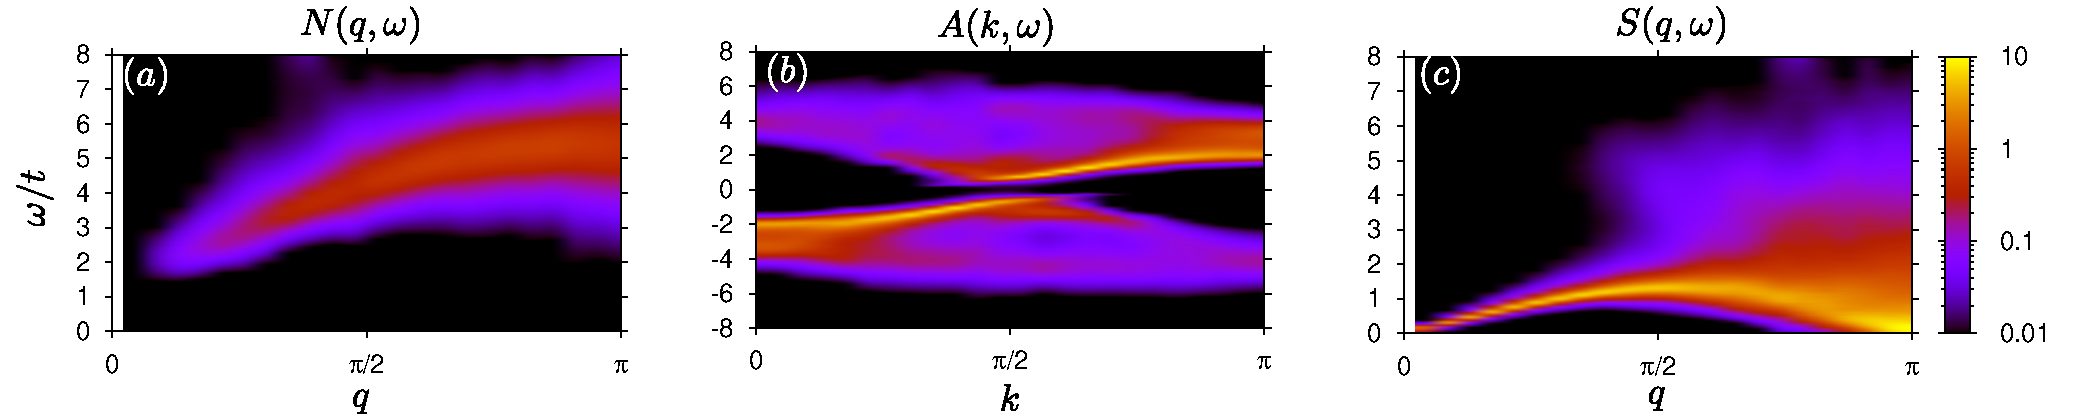
\includegraphics[width=\textwidth,clip]{Figures/MaxEnt/Spectral_1D.pdf}

\caption{Dynamics of the one-dimensional half-filled Hubbard model  on a 46-site chain   and at U/t=4 and at $\beta t = 10$.  (a) Dynamical charge structure factor, (b) single particle spectral function and (c) dynamical spin structure factor.   As apparent in the pyALF python script 
 \href{https://git.physik.uni-wuerzburg.de/ALF/ALF/-/blob/master/Documentation/Figures/MaxEnt/Hubbard_1D.py}{\texttt{Hubbard\_1D.py}}  we consider 400  bins of 200 sweeps  each and  take into account the covariance matrix for the MaxEnt.  The parameters for the MaxEnt  that differ for the default values are also listed in the  python script.}
        \label{Fig:Spectral1D}
\end{figure}
